\documentclass[10pt,twocolumn,letterpaper]{article}

\usepackage{cvpr}
\usepackage{times}
\usepackage{epsfig}
\usepackage{graphicx}
\usepackage{amsmath}
\usepackage{amssymb}
\usepackage{listings}
\usepackage{subcaption}
\usepackage{lipsum}
\usepackage{color} %red, green, blue, yellow, cyan, magenta, black, white
\definecolor{mygreen}{RGB}{28,172,0} % color values Red, Green, Blue
\definecolor{mylilas}{RGB}{170,55,241}
\lstset{language=Matlab,%
    %basicstyle=\color{red},
    breaklines=true,%
    morekeywords={matlab2tikz},
    keywordstyle=\color{blue},%
    morekeywords=[2]{1}, keywordstyle=[2]{\color{black}},
    identifierstyle=\color{black},%
    stringstyle=\color{mylilas},
    commentstyle=\color{mygreen},%
    showstringspaces=false,%without this there will be a symbol in the places where there is a space
    numbers=left,%
    numberstyle={\tiny \color{black}},% size of the numbers
    numbersep=9pt, % this defines how far the numbers are from the text
    emph=[1]{for,end,break},emphstyle=[1]\color{red}, %some words to emphasise
    %emph=[2]{word1,word2}, emphstyle=[2]{style},
}

% Include other packages here, before hyperref.

% If you comment hyperref and then uncomment it, you should delete
% egpaper.aux before re-running latex.  (Or just hit 'q' on the first latex
% run, let it finish, and you should be clear).
 
\usepackage[pagebackref=true,breaklinks=true,letterpaper=true,colorlinks,bookmarks=true,bookmarksnumbered=true,hypertexnames=false,linkbordercolor={0 0 1}]{hyperref}
% Include other packages here, before hyperref.

% If you comment hyperref and then uncomment it, you should delete
% egpaper.aux before re-running latex.  (Or just hit 'q' on the first latex
% run, let it finish, and you should be clear).
%\usepackage[pagebackref=true,breaklinks=true,letterpaper=true,colorlinks,bookmarks=false]{hyperref}

\cvprfinalcopy % *** Uncomment this line for the final submission

\def\cvprPaperID{****} % *** Enter the CVPR Paper ID here
\def\httilde{\mbox{\tt\raisebox{-.5ex}{\symbol{126}}}}

% Pages are numbered in submission mode, and unnumbered in camera-ready
\ifcvprfinal\pagestyle{empty}\fi
%\setcounter{page}{1}
\begin{document}

%%%%%%%%% TITLE
\title{Automatic Face Replacement on a Morphing Model}

\author{Han Li\\
Department of Computer Sciences\\
University of Wisconsin-Madison\\
{\tt\small hli337@wisc.edu}
% For a paper whose authors are all at the same institution,
% omit the following lines up until the closing ``}''.
% Additional authors and addresses can be added with ``\and'',
% just like the second author.
% To save space, use either the email address or home page, not both
\and
Wentao Wu\\
Department of Computer Sciences\\
University of Wisconsin-Madison\\
{\tt\small wwu69@wisc.edu}
}

\maketitle
%\thispagestyle{empty}

%%%%%%%%% ABSTRACT
\begin{abstract}
   With the unprecedented and exponentially increasing of web images and videos,  there is a growing concern of online iconographic privacy. Thus, editing and rewriting these image-based media resources is becoming an interesting and urgent task. In this project, we propose a new automatic face replacement in a resource (image or video) based on face morphing and blending from an existing facial data resource. The procedure consists of four steps: (1) face recognition and landmark representation based on a third party computer vision library, Face $++$, (2) face morphing using Thin-Plate-Spline method, (3) optimal image seam searching based on a graph-cut algorithm, and (4) face blending with color and illumination adjusting based on Poisson blending. We conduct face replacement tasks on both images and videos. The empirical experiments show that the results not only look natural to human judgements but also can handle the facial expressions well, and proved the effectiveness of the method.
\end{abstract}
%%%%%%%%% BODY TEXT
\section{Introduction}

With the unprecedented and exponentially increasing of high-definition web images and videos, online iconographic privacy is becoming a severe problem and concerned by more and more people. For example, online systems such as Google Street View allow users to browse photos of public images possibly containing many people who might not consent to be photographed. However, currently Google solves this problem by using blur masks, which is a typical, low-cost way but makes the image looks pretty ugly. Fig. \ref{fig:gsv} shows an example from Google Street View that contains a child face with blur mask. Thus, it becomes more and more urgent and popular to develop face replacement techniques to alleviate this problem. In this project, we propose a new face replacement method based on a shape-morphing model for image and video facial information hiding. Given a source image and a target resource (image or video), the pipeline contains four steps:
\begin{enumerate}
 \item face detection and landmark localization based on Face ++, a third party library focusing on computer vision;
 \item face morphing according to the landmarks by Thin-Plate-Spline method to fit the source face into the target image;
 \item optimal seam searching to include the most important part of the face;
 \item face blending with possible color and illumination adjusting to make the synthesized face look natural.
 \end{enumerate}
 We test our method on a set of images and two videos. The empirical experiments show that the results look natural to human judgements. Also, since many of the previous methods haven't cared much about the facial expressions, our method could handle them well, and thus the contribution of this project would be integrating the facial expression into the face replacement procedure.

\begin{figure}[t]
\begin{center}
%\fbox{\rule{0pt}{2in} \rule{0.9\linewidth}{0pt}}
   \includegraphics[width=0.8\linewidth]{fig/fig1.png}
\end{center}
   \caption{An image from Google Street View that contains a human face with blur mask.}
\label{fig:gsv}
\end{figure}

\indent We organize the paper as follow. We introduce the background and some related work in Section \ref{sec:relatedwork}, describe each of the pipeline steps in detail from Section \ref{sec:landmark} to Section \ref{sec:blending}. We show our experimental results in Section \ref{sec:experiment}. And finally, we make the conclusion and prospect some future work in Section \ref{sec:conclusion}.

%------------------------------------------------------------------------
\section{Related Work}
\label{sec:relatedwork}
Our project is most related to Min's work \cite{min2010automatic}. They proposed an automatic face
replacement approach in video based on 2D Morphable model. This approach includes three main modules: face alignment, face morph, and face fusion. They use the Active Shape Models (ASM) for face alignment. They also consider color and lightning adjustment to keep consistent. Their approach is fully automatic without user interference, and generates natural and realistic results. Furthermore, as they use 2D model, their algorithm is also efficient. However, they don't consider facial expression. The tolerance to pose and expression variance is limited by ASM.

Liang \cite{liang2009image} proposed a video face replacement system which allows replacing target human face from
target video with source face in source video. For each target face in target video, they select the best candidate face with similar face expression. Finally, they blend candidate replacement to target video. In their approach, however, they require the target video should have similar face expression and pose with the source video. 

Similar to Liang's work, Dale \cite{dale2011video} also proposed an algorithm to provides face replacement in target video from source video. They tracks both faces in target and source video using multilinear model. Using this tracked 3D Geometry, source face is warped to target face in every frame of video. But, their tracking algorithm is based on optical flow, so the light should change slowly in the video.

Afifi \cite{afifi2014video} presented a system for video face replacement that requires only two videos of a source actor and a target actor using only a single digital camera. They could generate realistic results without using special equipment and 3D model. Also, they use a new face blending technique based on poisson blending. But their algorithm only works for fixed pose, i.e. front face.

Instead of using source video, Cheng \cite{cheng20093d} uses only two face pictures: one frontal view and one profile view. First, they use these two images to construct 3D face model. Then, they track the faces in the video and project the source face model to align and replacement the faces in target video. However, the tolerance to the pose is limited to robustness of their alignment algorithm.

A. Niswar \cite{niswar2012face} proposed a system where one image is required to replace the faces in target video. Also, the image is not limited a specific pose. There are four steps in their approach: 3D face reconstruction, 3D face animation, feature points tracking, 2D projection with blending. Their approach, however, has high complexity and hence high time consuming. 

%------------------------------------------------------------------------
\section{Landmark Localization}
\label{sec:landmark}
To replace a face in an image, the first thing we need to do is to recognize the face(s) in the given image. In this project, we use \emph{landmarks} as the representation of a face. The landmarks are a set of key points on a face that sketch the outline of a face. Fig. \ref{fig:landmark} shows an example of landmarks in a face. There are two reasons we use landmarks. First, we can use the convex hull of the landmarks as the face region recognition. A more important reason is that landmarks provide us the anchors for face morphing in the next step, which would be explained in detail in the next section. 

Since the landmark localization is the fundamental step of our pipeline, and the quality of the landmarks would influence the performance of our method greatly, in this project we choose to use a third party library, Face $++$\footnote[1]{http://www.faceplusplus.com/}, for this task. The Face $++$ landmark localizer is based on a deep convolutional neural network proposed by Zhou \etal \cite{zhou2013extensive}, and for each image, it provides $83$ landmarks. Fig. \ref{fig:facepp} shows the system workflow. The basic idea is to use $4$ hidden layers to refine the results.  The first level networks predict the bounding boxes for the inner points and contour points separately. For the inner points, the second level predicted a initial estimation of the positions which are refined by the third level for each component. The fourth level is used to further improve the predictions of mouth and eyes by taking the rotated image patch as input. Two levels are used
for contour points. Currently, the Face $++$ achieves the state-of-the-art performance on landmark localization.

\begin{figure}[t]
\begin{center}
%\fbox{\rule{0pt}{2in} \rule{0.9\linewidth}{0pt}}
   \includegraphics[width=0.8\linewidth]{fig/landmark.png}
\end{center}
   \caption{Landmarks in a human face. The landmark point set contains face contour, nose, mouth, eyes, and eyebrows.}
\label{fig:landmark}
\end{figure}

Because Face $++$ is not open source, we use the matlab API to landmark localizer which uploads the image to the server and returns the coordinates of the landmarks in the image. The code
can be downloaded directly from the website \footnote[2]{http://www.faceplusplus.com/dev-tools-sdks/}.

\begin{figure*}
\begin{center}
%\fbox{\rule{0pt}{2in} \rule{.9\linewidth}{0pt}}
   \includegraphics[width=0.8\linewidth]{fig/facepp.png}
\end{center}
   \caption{System workflow of Face $++$.}
\label{fig:facepp}
\end{figure*}
%------------------------------------------------------------------------
\section{Face Morphing}
\label{sec:morphing}
Based on the landmarks generated from the first step, the next thing to do is face morphing. The reason we need to perform morphing is that people have different faces, e.g. different shape of contour, size of eyes, size of nose. Even if we have the convex hull of the face contour from the landmarks, we cannot directly replace old face with the new one without any morphing. We need to change the structure of the face to make sure that the components in the new face have the similar relative distance from each other as in the old face.

To achieve this goal, we choose to use Thin-Plate-Spline (TPS) method. TPS is an interpolation method for non-rigid surface morphing. Here the name "thin plate" refers to a physical analogy involving the bending of a thin sheet of metal to get the non-rigid surface morphing. Given a set of $2$D data points, the basic idea of TPS is to produce a weighted combination of thin plate splines centered at each designated point which gives the interpolation function that passes through the points exactly and also minimizes the \emph{blending energy} of the surface. Here the blending energy is defined as follow:

\begin{equation*}
I[f(x, y)] = \int\int_{R^2}(f_{xx}^2 + 2f_{xy}^2 + f_{yy}^2)dxdy
\end{equation*}

There are three reasons that we select TPS for face morphing: (1) TPS produces non-rigid, smooth surface morphing which is required by our task; (2) there are no free parameters in TPS that need manual tuning; (3) TPS has closed-form solutions for parameter estimation and morphing, which guarantees the performance and also the training speed.

In the face replacement scenario, to morph the source face to the target one, there are two steps: first, align all of the source landmarks to the corresponding target ones to get the interpolation functions; second, perform TPS morphing based on the interpolation functions. Formally, given the source landmark vector $P_{src} = (s_1, ..., s_K)$, target landmark vector $P_{tgt} = (t_1, ..., t_K)$ with $K$ landmarks each, and function $U(r) = r^2 \log r^2$ with $r = \sqrt{x^2 + y^2}$, we need to solve the following equation:
\begin{equation}
\label{eq1}
\begin{bmatrix}
K & P_{src} \\
P_{src}^\top & 0
\end{bmatrix}
\begin{bmatrix}
w \\
a 
\end{bmatrix}
= 
\begin{bmatrix}
P_{tgt} \\
0
\end{bmatrix}
\end{equation}
where $w$ and $a$ are the model parameters that we need to estimate, and 
\begin{equation*}
K_{ij} = U(||(x_{src, i}, y_{src, i}) - (x_{src, j}, y_{src, j})||)
\end{equation*}
Note that we could expand Eq. \ref{eq1} to get the following form:
\begin{equation}
\label{eq2}
f(x, y) = a_1 + a_xx + a_yy + \sum_{i=1}^pw_iU(||(x_{i}, y_{i}) - (x_{j}, y_{j})||)
\end{equation}
thus once we get the parameter estimation from Eq. \ref{eq1}, we could fit the parameters into Eq. \ref{eq2} and perform the point morphing in the whole image. 

Fig. \ref{fig:morphing} shows an example of face morphing after applying TPS model. Now we can see that the new morphed face is pretty similar to the target one with respect to the face components, and could fit into the new image perfectly.
\begin{figure*}
\begin{center}
%\fbox{\rule{0pt}{2in} \rule{.9\linewidth}{0pt}}
   \includegraphics[width=0.8\linewidth]{fig/morphing.png}
\end{center}
   \caption{An example of face morphing.}
\label{fig:morphing}
\end{figure*}
%------------------------------------------------------------------------
\section{Optimal Seam Searching}
\label{sec:searching}
After we warped the two images, we need to find an optimal seam. A seam is a series of continuous pixels along which the area extracted from the source image can be determined. There are three main concerns for the optimal search. First, we want to avoid the the important features in face, such as eyes, mouth, nose and so on. Second, the pixels on the boundary of the extracted area should be similar between the two images so that it will look more natural when we composite them together. Third, we want to reduce the computation complexity.


\begin{figure}[hb]
  \centering
  \includegraphics[width=0.4\textwidth]{graph_image.png}
  \caption{Graph representation of image, from \cite{kwatra2003graphcut}}\label{graph}
\end{figure}


Our approach is based on Kwatra et al's work \cite{kwatra2003graphcut}. The algorithm works by formulating the image as a connected graph with edge weights based on the difference between neighboring pixels. This graph is then treated as a max-flow/min-cut problem where the sources are any pixels to be taken only from the first image and the sinks are any pixels to be taken only from the second image.

As the figure \ref{graph} shows, in our project, the pixels in patch A must from our target image while the pixels in patch B must from source image. The goal is to find the optimal cut between patch A and patch B. We represent the image graph as an adjacency matrix while each entry in the adjacency matrix can be the flow. We use the sum of absolute difference between the source image and the target image plus the sum of absolute difference of the source image and the target image at the neighboring pixel.

\begin{equation}
M(c,n,S,T) = \Vert S(c) - T(c) \Vert_1 + \Vert S(n) - T(n) \Vert_1
\end{equation}

where $c$ is the current pixel, $n$ is the neighbor pixel, $S$ is the source image and $T$ is the target image. The $L1$ norm is the sum of absolute difference of these two pixels in three channels. Note that the weight between the pixels in patch A and its neighbors must be infinity. This is same for patch B.

In our implementation, we first define the permissible path region by generating two masks based on the landmarks generated from the first step, as shown in \ref{seam-mask}. The permissible path region is the area we want to find the optimal cut. All the pixels which are outside the right larger mask must from target image, i.e. patch B, and all the pixels inside the left smaller mask must from source image, i.e. patch A. Therefore, the permissible path region is the area which is inside the larger mask but outside the smaller mask. A good permissible region is crucial for the following steps. The permissible path should not be too strict, then it's highly possible that we cannot find the optimal seam within the strict area. Also, the larger the permissible path region is, the higher computation complexity will be. When constructing the two masks, a convex hull is constructed by the landmarks. As the forehead region of a face is usually more flat than the other regions, we split the face into two regions: the forehead region and the bottom region. For the forehead region, as the convex hull is right above the eyes, the mask is eroded so that the permissible path region will cover larger area. For the bottom region, the convex hull is almost at the boundary of the face, so it is not reasonable to extend the permissible path outside the face, the mask is dilated. After generating two masks for each region via erosion and dilation, we stitch them together to get the final permissible path region.

For the construction of the adjacency matrix, we extend the patch A and patch B by including all the pixels which are immediate neighbors. In other words, if the neighbor of a pixel is in patch A or B, then the weight between them is also infinite. If the weight between two pixels is not infinite, then these two pixels must be 1) not in patch A and patch B and 2) their neighbors are also not in patch A and patch B.

\begin{figure}[h]
  \centering
  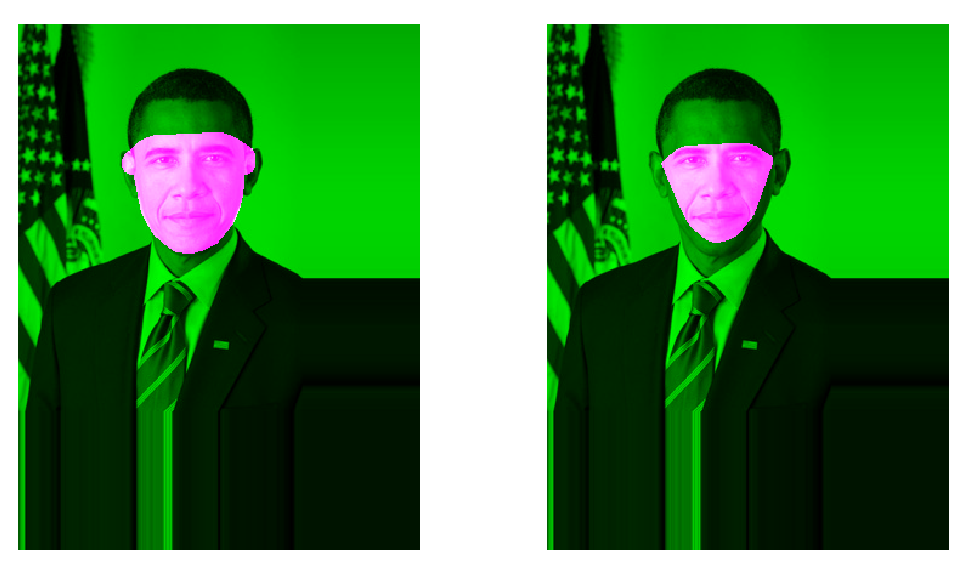
\includegraphics[width=0.4\textwidth]{seam_mask.eps}
  \caption{Mask for optimal seam search}\label{seam-mask}
\end{figure}

The result is shown in Fig.\ref{seam-result}. The pink area is the permissible path region and the red circle in the left figure is the result.

\begin{figure}[h]
  \centering
  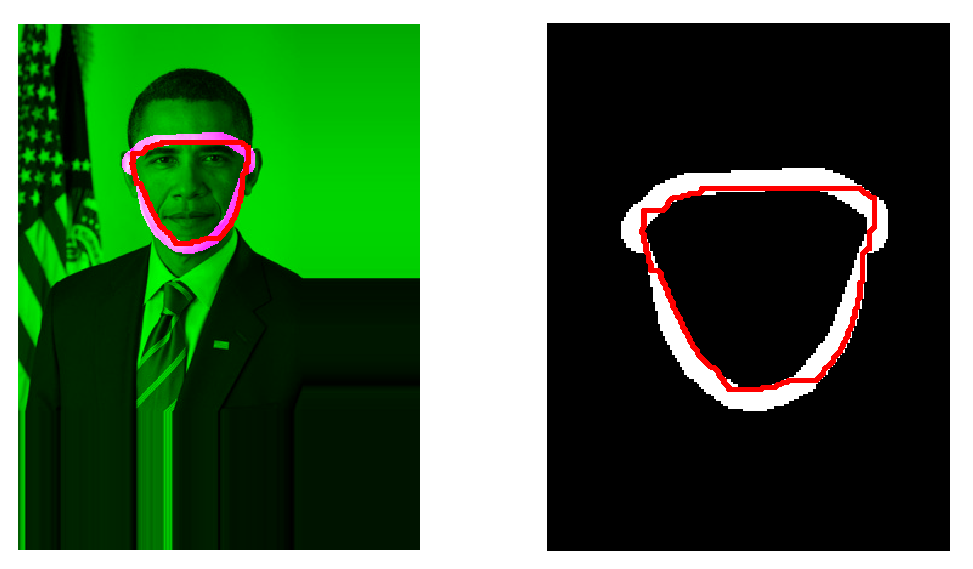
\includegraphics[width=0.4\textwidth]{seam_result.eps}
  \caption{Result for optimal seam search}\label{seam-result}
\end{figure}

%------------------------------------------------------------------------
\section{Face Blending}
\label{sec:blending}
The optimal seam tells us what is the best area which should be extract from the source image. If we simply cut that area from the source image and paste it to the target image, the result will not be satisfiable, as the left image shown in Fig\ref{blending}. The problem is the color of these two images are very different from each other. Therefore, we can see the color change abruptly around the boundary. In order to avoid the abrupt color changes, we use Poisson blending approach.

\begin{figure}[h]
  \centering
  \includegraphics[width=0.4\textwidth]{poisson_blending_alg.png}
  \caption{Poisson blending notation, \cite{perez2003poisson} }\label{blending_alg}
\end{figure}

Poisson blending is one of gradient domain image processing methods. As Fig.\ref{blending_alg} shown, $v$ is gradient of a region in an image, $g$ is selected region of source, $f^*$ is a known functions that exist in domain $S$, $f$ is an unknown functions that exist in domain $\Omega$, $\Omega$ is a region $g$ that is now placed on domain $S$ (target background), $\partial{\Omega}$ is boundaries between the source and target regions. The goal is given $v$, find the value of $f$ in the unknown region that optimize

\begin{eqnarray}
min_{f} & \iint_{\Omega} \vert \nabla f -v \vert^2  \\
\mbox{subject to} & f \mid_{\partial{\Omega}} = f^* \mid_{\partial{\Omega}}
\end{eqnarray}
where $\nabla = [\frac{\partial{}}{\partial{x}}, \frac{\partial{}}{\partial{y}}]$ is the gradient vector. Its solution is the unique solution of the following Poisson equation with Dirichlet boundary conditions:

\begin{eqnarray}
& \Delta f = \mbox{div }v \quad \mbox{over } \Omega \\
\mbox{subject to} & f \mid_{\partial{\Omega}} = f^* \mid_{\partial{\Omega}}
\end{eqnarray}
where $\mbox{div} v = \frac{\partial{u}}{\partial{x}} + \frac{\partial{v}}{\partial{x}}$ is the divergence of $v = (u,v)$, and $\Delta$ is the Laplacian operator as Matrix \ref{lap} shown.

\begin{table}[h!]
\centering
\begin{tabular}{|l|l|l|}
\hline
 0 & -1 & 0 \\ \hline
 -1 & 4 & -1  \\ \hline
 0 & -1 & 0  \\ \hline
\end{tabular}
\caption{Laplacian Operator}
 \label{lap}
\end{table}

\begin{figure}[h]
  \centering
  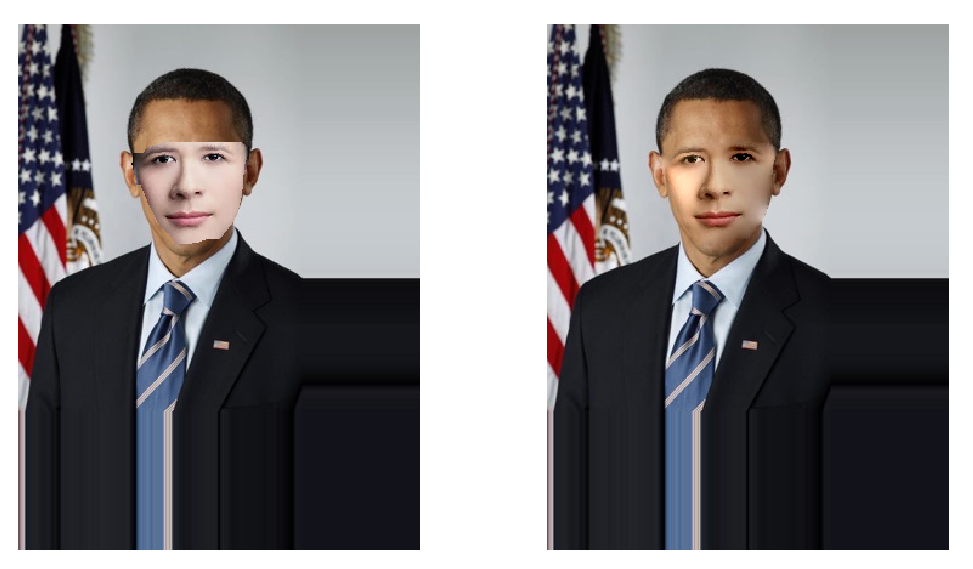
\includegraphics[width=0.4\textwidth]{possion_blending_result.eps}
  \caption{Poisson blending}\label{blending}
\end{figure}

This is the fundamental machinery of Poisson editing of color images: three Poisson equations of the above equation are solved independently in the three color channels of the chosen color space. The result is shown in the left image in Fig.\ref{blending}.

%------------------------------------------------------------------------
\section{Experiments}
\label{sec:experiment}
We tested our algorithm with various images. The results are shown in Fig.\ref{result} and Fig.\ref{more_result}. Each example shows, from left to right, the source image, the target image and the composite image. Note that even the skin color in the source image and target are different, the skin color in composite image looks quite natural by using Poisson blending as shown in Fig.\ref{fig:eg1}. One issue in previous work is that it's usually difficult to handle the different expressions in the source and target image. In our approach, using Thin-Plate-Spline method after extracting the facial landmarks, the source image can be morphed to the target image perfectly even the two images have quite different facial expression, as shown in Fig.\ref{fig:eg2}. Note that the mouth in the target image is open while it is closed in the source image.

If the face is covered by some objects, such as hair or hands, our approach may not generate satisfiable results. As Fig.\ref{fig:eg3} shows, part of the face in the target image is covered by her hair. In the composite image, that part of hair is replaced by the face from the source image. This is because we construct the masks based on the facial landmarks and we assume the whole face, i.e. the convex hull of the landmarks, appears in the image. If this assumption is violated, the composite image will look unnatural.

\begin{figure}
\centering
   \begin{subfigure}[b]{0.4\textwidth}
   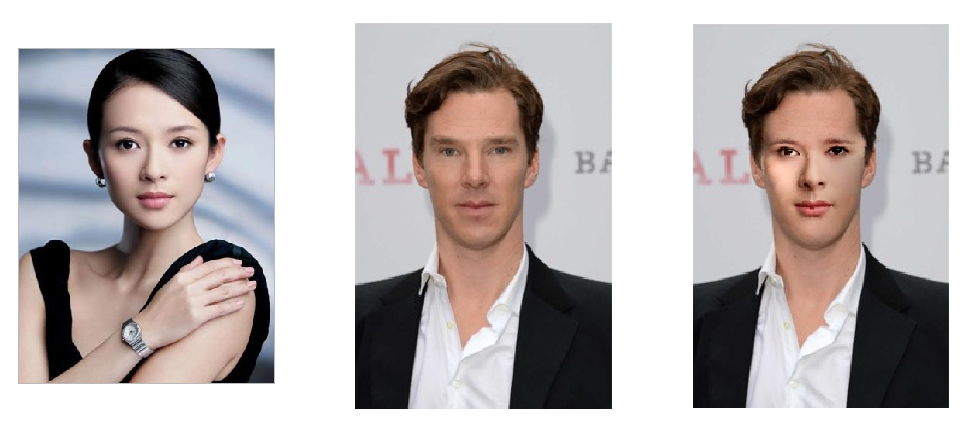
\includegraphics[width=1\linewidth]{3_4.eps}
   \caption{Result 1: front face}
   \label{fig:eg1}
\end{subfigure}

\begin{subfigure}[b]{0.4\textwidth}
   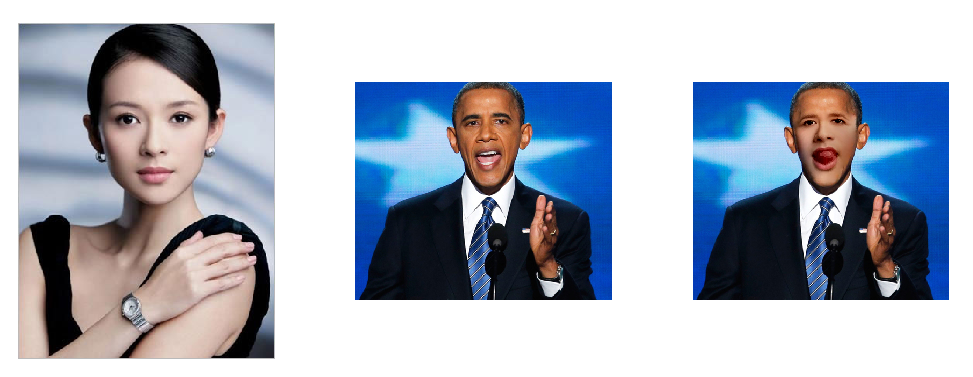
\includegraphics[width=1\linewidth]{3_10.eps}
   \caption{Result 2: different expression}
   \label{fig:eg2}
\end{subfigure}
\begin{subfigure}[b]{0.4\textwidth}
   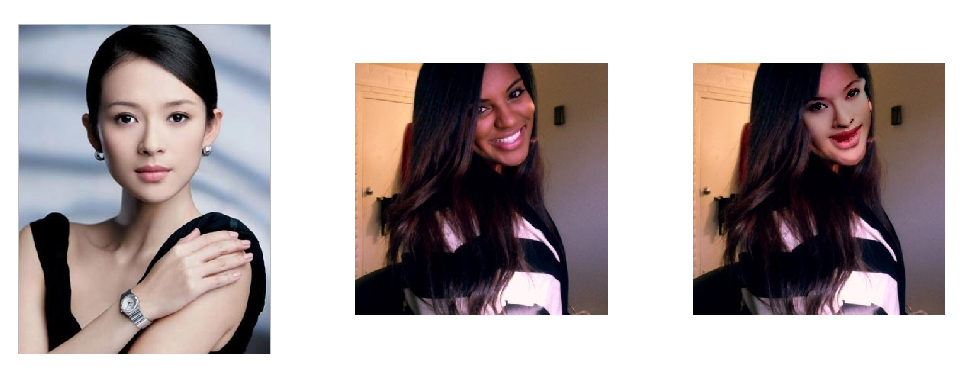
\includegraphics[width=1\linewidth]{3_9.eps}
   \caption{Result 3: part face}
   \label{fig:eg3}
\end{subfigure}
\caption{Results}\label{result}
\end{figure}

\begin{figure}
\centering
   \begin{subfigure}[b]{0.4\textwidth}
   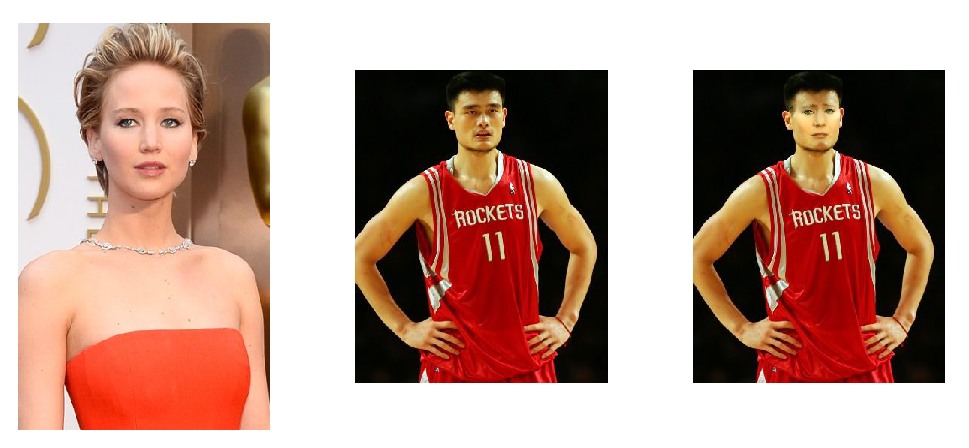
\includegraphics[width=1\linewidth]{7_8.eps}
   \label{fig:eg4}
\end{subfigure}

\begin{subfigure}[b]{0.4\textwidth}
   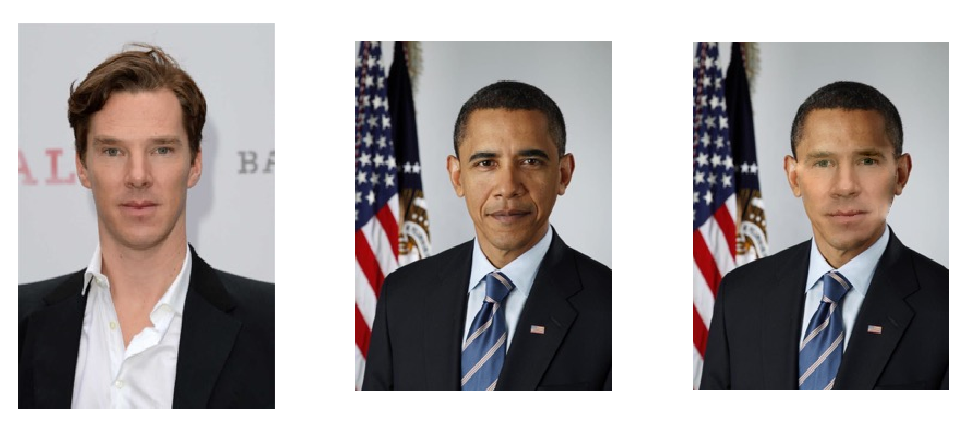
\includegraphics[width=1\linewidth]{4_5.eps}
   \label{fig:eg5}
\end{subfigure}
\begin{subfigure}[b]{0.4\textwidth}
   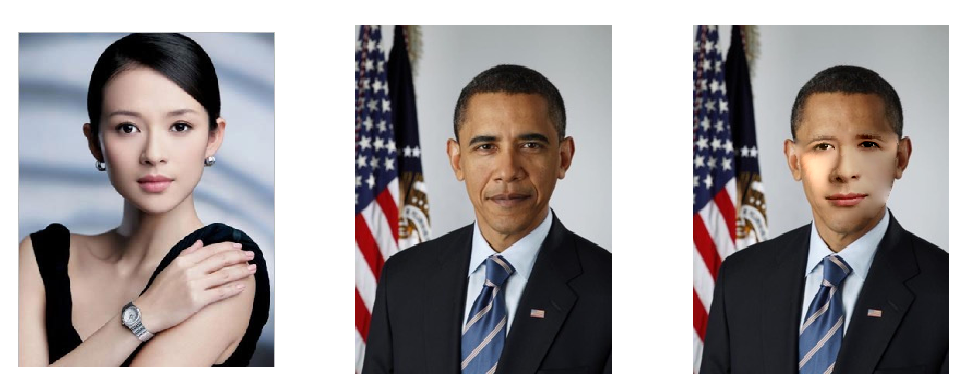
\includegraphics[width=1\linewidth]{3_5.eps}
   \label{fig:eg6}
\end{subfigure}
\caption{More Results}\label{more_result}
\end{figure}

%------------------------------------------------------------------------
\section{Conclusion and Future Work}
\label{sec:conclusion}
In this project, we propose a new automatic face replacement method based on Thin-Plate-Spline morphing algorithm. The method is fully automated without any human intervention, and the four-step pipeline guarantees the performance of the procedure. The empirical experiments show that this new method could fit a source face into the target image effectively and also capture the facial expressions, thus does a perfect job on front face replacement both in images and videos.

To make the method even more powerful, several improvements can be done in future. First, currently we just use one image as the source image, and it would inevitably cause the bad performance on side face morphing. To alleviate this, we could instead use a set of images containing different poses. Second, because the Face $++$ cannot recognize some side faces, and thus leads to discontinuous frames in the video face replacement, in future we could use some interpolation methods to plug in the missing frames using the neighborhoods. Finally, a better color adjustment might be invented for better image blending.

{\small
\section*{Acknowledgments}
We thank Prof. Singh and TA Jia for their devotion and meticulous guidance during this semester.
}

{\small
\bibliographystyle{ieee}
\bibliography{report}
}


\end{document}
